\documentclass{standalone}
\usepackage{tikz}
\usetikzlibrary{backgrounds}
\begin{document}
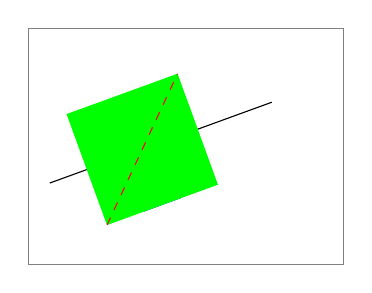
\begin{tikzpicture}
  \draw[gray] (0,0) rectangle (4,3);
  \begin{scope}[shift={(1,0.5)}, rotate=20, red, line width=2pt, dashed]
    \clip (0,0) rectangle (1.5,1.5);
    \fill[green] (-1,-1) rectangle (3,3);
    \begin{pgfonlayer}{background}
      % Transformed like the scope, but not clipped, black, 0.4pt and solid.
      \draw (-0.5,0.75) -- (2.5,0.75);
      \begin{scope}[blue, xshift=0.5cm]
        \fill (0,0) rectangle (0.5,0.5);
      \end{scope}
    \end{pgfonlayer}
    \draw (0,0) -- (2,2);
  \end{scope}
\end{tikzpicture}
\end{document}
